\chapter{Conclusion}
brief of conclusion

\section{Ahmad Syafrizal Huda/1164062}
\subsection{Teori}
\begin{enumerate}
\item Jelaskan Kenapa Kata-Kata harus dilakukan vektorisasi lengkapi dengan ilustrasi gambar.
\subitem Kata kata harus dilakukan vektorisasi dikarenakan untuk mengukur nilai kemunculan suatu kata yang sama dari sebuah kalimat sehingga kata-kata tersebut dapat di prediksi berapa kemunculanya. Atau juga di buatkan vektorisasi data yang digunakan untuk memprediksi bobot dari suatu kata misalkan mobil dan motor sama-sama kendaraan maka akan dibuat prediksi apakah kata tersebut akan muncul pada kalimat yang kira-kira memiliki bobot yang sama. 
\par Untuk ilustrasinya dapat dilihat pada gambar \ref{c5_1}
\begin{figure}[!htbp]
	\centerline{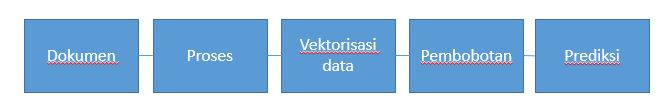
\includegraphics[width=1\textwidth]{figures/huda/chapter5/1.JPG}}
	\caption{Ilustrasi Soal No. 1}
	\label{c5_1}
\end{figure}
\item Jelaskan Mengapa dimensi dari vektor dataset google bisa mencapai 300 lengkapi dengan ilustrasi gambar.
\subitem Dimensi dari vektor dataset google bisa mencapai 300 karena dimensi dari vektor digunakan untuk membandingkan bobot dari setiap kata, misalkan terdapat kata mobil dan motor pada dataset google tersebut setiap kata tersebut di buat dimensi vektor 300 untuk kata mobil dan 300 dimensi vektor juga untuk kata motor kemudian kata tersebut di bandingkan bobot kesamaan katanya maka akan muncul akurasi sekitar 70an persen kesamaan bobot dikarenakan kata mobil dan motor sama sama di gunakan sebagai kendaraan.
\par Untuk ilustrasinya dapat dilihat pada gambar \ref{c5_2}
\begin{figure}[!htbp]
	\centerline{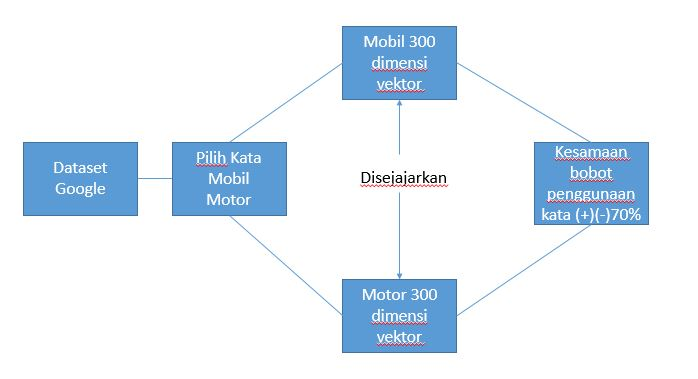
\includegraphics[width=1\textwidth]{figures/huda/chapter5/2.JPG}}
	\caption{Ilustrasi Soal No. 2}
	\label{c5_2}
\end{figure}
\item Jelaskan Konsep vektorisasi untuk kata . dilengkapi dengan ilustrasi atau gambar.
\subitem Konesp vektorisasi untuk kata yaitu mengetahui kata tengah dari suatu kalimat utama dengan suatu kalimat contoh ( Jangan lupa like dan comment yah makasih ) kata tengah tersebut merupakan (dan) yang memiliki bobot sebagai kata tengah dari suatu kalimat atau bobot sebagai objek dari suatu kalimat. hal ini sangat berkaitan dengan dimensi vektor pada dataset google yang 300 tadi karena untuk mendapatkan nilai atau bobot dari kata tengah tersebut di dapatkan dari proses dimensiasi dari kata tersebut. 
\par Untuk ilustrasinya dapat dilihat pada gambar \ref{c5_3}
\begin{figure}[!htbp]
	\centerline{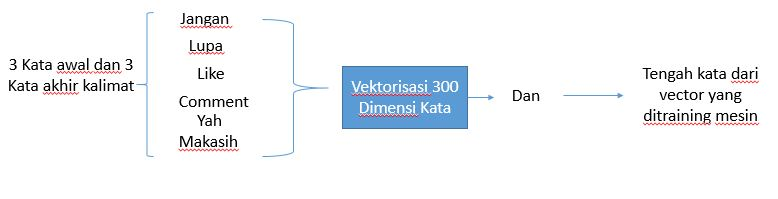
\includegraphics[width=1\textwidth]{figures/huda/chapter5/3.JPG}}
	\caption{Ilustrasi Soal No. 3}
	\label{c5_3}
\end{figure}
\item Jelaskan Konsep vektorisasi untuk dokumen. dilengkapi dengan ilustrasi atau gambar.
\subitem Konsep vektorisasi untuk dokumen hampir sama seperti vektorisasi untuk kata hanya saja pemilihan kata utama atau kata tengah terdapat pada satu dokumen jadi mesin akan membuat dimensi vektor 300 untuk dokumen dan nanti kata tengahnya akan di sandingkan pada dokumen yang terdapat pada dokumen tersebut.
\par Untuk ilustrasinya dapat dilihat pada gambar \ref{c5_4}
\begin{figure}[!htbp]
	\centerline{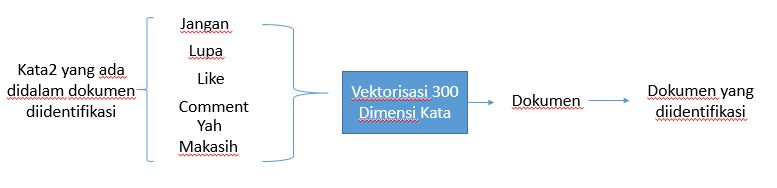
\includegraphics[width=1\textwidth]{figures/huda/chapter5/4.JPG}}
	\caption{Ilustrasi Soal No. 4}
	\label{c5_4}
\end{figure}
\item Jelaskan apa mean dan standar deviasi, lengkapi dengan iludtrasi atau gambar.
\subitem Mean adalah nilai rata-rata dari suatu data. Mean disini merupakan petunjuk terhadap kata-kata yang di olah jika kata kata itu akurasinya tinggi berarti kata tersebut sering muncul begitu juga sebaliknya. Standar deviasi merupakan standar untuk menimbang kesalahan. Misalkan kita memperkirakan kedalaman dari dataset merupakan 2 atau 3 tapi pada kenyataanya merupakan 5 itu merupakan kesalahan tapi masih bisa dianggap wajar karena masih mendekati perkiraan awal.
\par Untuk ilustrasinya dapat dilihat pada gambar \ref{c5_5}
\begin{figure}[!htbp]
	\centerline{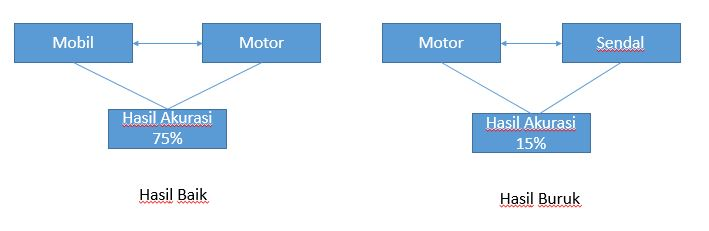
\includegraphics[width=1\textwidth]{figures/huda/chapter5/5.JPG}}
	\caption{Ilustrasi Soal No. 5}
	\label{c5_5}
\end{figure}
\item Jelaskan Apa itu Skip-Gram sertakan contoh ilustrasi.
\subitem Skip-Gram yaitu dimana kata tengah menjadi acuan terhadap kata kata pelengkap dalam suatu kalimat.
\par Untuk ilustrasinya dapat dilihat pada gambar \ref{c5_6}
\begin{figure}[!htbp]
	\centerline{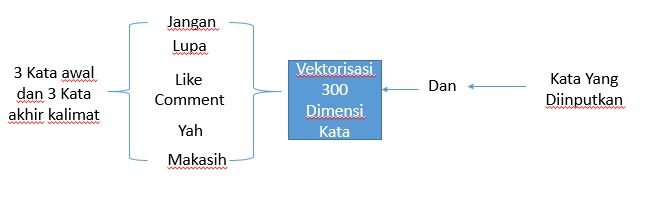
\includegraphics[width=1\textwidth]{figures/huda/chapter5/6.JPG}}
	\caption{Ilustrasi Soal No. 6}
	\label{c5_6}
\end{figure}
\end{enumerate}

\subsection{Praktek Program}
\begin{enumerate}
\item Cobalah dataset google, dan jelaskan vektor dari kata love, faith, fall, sick, clear, shine, bag, car, wash, motor, cycle dan cobalah untuk melakukan perbandingan similirati dari masing-masing kata tersebut. Jelaskan arti dari outputan similaritas.
\subitem Output source code dibawah akan memunculkan data vektor untuk kata love. bahwa vektor memiliki array sebanyak 300 dimensi. Hasil pada source code tersebut dapat dilihat pada gambar \ref{c5_7}.
\begin{verbatim}
gmodel['love']
\end{verbatim}
\begin{figure}[!htbp]
	\centerline{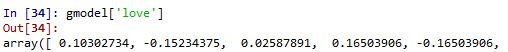
\includegraphics[width=1\textwidth]{figures/huda/chapter5/7.JPG}}
	\caption{Love}
	\label{c5_7}
\end{figure}
\subitem Output source code dibawah akan memunculkan data vektor untuk kata faith. bahwa vektor memiliki array sebanyak 300 dimensi. Hasil pada source code tersebut dapat dilihat pada gambar \ref{c5_8}.
\begin{verbatim}
gmodel['faith']
\end{verbatim}
\begin{figure}[!htbp]
	\centerline{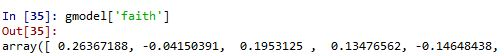
\includegraphics[width=1\textwidth]{figures/huda/chapter5/8.JPG}}
	\caption{Faith}
	\label{c5_8}
\end{figure}
\subitem Output source code dibawah akan memunculkan data vektor untuk kata fall. bahwa vektor memiliki array sebanyak 300 dimensi. Hasil pada source code tersebut dapat dilihat pada gambar \ref{c5_9}.
\begin{verbatim}
gmodel['fall']
\end{verbatim}
\begin{figure}[!htbp]
	\centerline{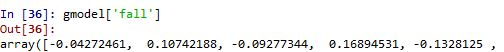
\includegraphics[width=1\textwidth]{figures/huda/chapter5/9.JPG}}
	\caption{Fall}
	\label{c5_9}
\end{figure}
\subitem Output source code dibawah akan memunculkan data vektor untuk kata sick. bahwa vektor memiliki array sebanyak 300 dimensi. Hasil pada source code tersebut dapat dilihat pada gambar \ref{c5_10}.
\begin{verbatim}
gmodel['sick']
\end{verbatim}
\begin{figure}[!htbp]
	\centerline{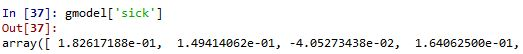
\includegraphics[width=1\textwidth]{figures/huda/chapter5/10.JPG}}
	\caption{Sick}
	\label{c5_10}
\end{figure}
\subitem Output source code dibawah akan memunculkan data vektor untuk kata clear. bahwa vektor memiliki array sebanyak 300 dimensi. Hasil pada source code tersebut dapat dilihat pada gambar \ref{c5_11}.
\begin{verbatim}
gmodel['clear']
\end{verbatim}
\begin{figure}[!htbp]
	\centerline{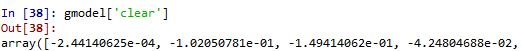
\includegraphics[width=1\textwidth]{figures/huda/chapter5/11.JPG}}
	\caption{Clear}
	\label{c5_11}
\end{figure}
\subitem Output source code dibawah akan memunculkan data vektor untuk kata shine. bahwa vektor memiliki array sebanyak 300 dimensi. Hasil pada source code tersebut dapat dilihat pada gambar \ref{c5_12}.
\begin{verbatim}
gmodel['shine']
\end{verbatim}
\begin{figure}[!htbp]
	\centerline{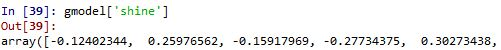
\includegraphics[width=1\textwidth]{figures/huda/chapter5/12.JPG}}
	\caption{Shine}
	\label{c5_12}
\end{figure}
\subitem Output source code dibawah akan memunculkan data vektor untuk kata bag. bahwa vektor memiliki array sebanyak 300 dimensi. Hasil pada source code tersebut dapat dilihat pada gambar \ref{c5_13}.
\begin{verbatim}
gmodel['bag']
\end{verbatim}
\begin{figure}[!htbp]
	\centerline{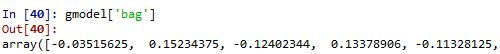
\includegraphics[width=1\textwidth]{figures/huda/chapter5/13.JPG}}
	\caption{Bag}
	\label{c5_13}
\end{figure}
\subitem Output source code dibawah akan memunculkan data vektor untuk kata car. bahwa vektor memiliki array sebanyak 300 dimensi. Hasil pada source code tersebut dapat dilihat pada gambar \ref{c5_14}.
\begin{verbatim}
gmodel['car']
\end{verbatim}
\begin{figure}[!htbp]
	\centerline{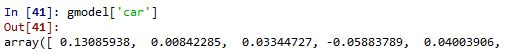
\includegraphics[width=1\textwidth]{figures/huda/chapter5/14.JPG}}
	\caption{Car}
	\label{c5_14}
\end{figure}
\subitem Output source code dibawah akan memunculkan data vektor untuk kata wash. bahwa vektor memiliki array sebanyak 300 dimensi. Hasil pada source code tersebut dapat dilihat pada gambar \ref{c5_15}.
\begin{verbatim}
gmodel['wash']
\end{verbatim}
\begin{figure}[!htbp]
	\centerline{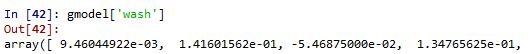
\includegraphics[width=1\textwidth]{figures/huda/chapter5/15.JPG}}
	\caption{Wash}
	\label{c5_15}
\end{figure}
\subitem Output source code dibawah akan memunculkan data vektor untuk kata motor. bahwa vektor memiliki array sebanyak 300 dimensi. Hasil pada source code tersebut dapat dilihat pada gambar \ref{c5_16}.
\begin{verbatim}
gmodel['motor']
\end{verbatim}
\begin{figure}[!htbp]
	\centerline{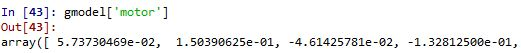
\includegraphics[width=1\textwidth]{figures/huda/chapter5/16.JPG}}
	\caption{Motor}
	\label{c5_16}
\end{figure}
\subitem Output source code dibawah akan memunculkan data vektor untuk kata cycle. bahwa vektor memiliki array sebanyak 300 dimensi. Hasil pada source code tersebut dapat dilihat pada gambar \ref{c5_17}.
\begin{verbatim}
gmodel['cycle']
\end{verbatim}
\begin{figure}[!htbp]
	\centerline{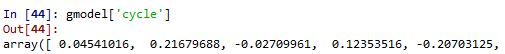
\includegraphics[width=1\textwidth]{figures/huda/chapter5/17.JPG}}
	\caption{Cycle}
	\label{c5_17}
\end{figure}
\subitem Pada source code dibawah menunjukkan hasil score perbandingan kata apakah kata motor dan cycle memiliki ke samaan atau tidak.  Hasil pada source code tersebut dapat dilihat pada gambar \ref{c5_18}.
\begin{verbatim}
gmodel.similarity('motor','cycle')
\end{verbatim}
\begin{figure}[!htbp]
	\centerline{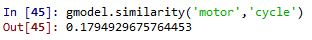
\includegraphics[width=1\textwidth]{figures/huda/chapter5/18.JPG}}
	\caption{Similariti Pada Kata Motor dan Cycle}
	\label{c5_18}
\end{figure}
\subitem Pada source code dibawah menunjukkan hasil score perbandingan kata apakah kata wash dan motor memiliki ke samaan atau tidak.  Hasil pada source code tersebut dapat dilihat pada gambar \ref{c5_19}.
\begin{verbatim}
gmodel.similarity('wash','motor')
\end{verbatim}
\begin{figure}[!htbp]
	\centerline{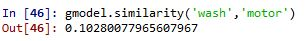
\includegraphics[width=1\textwidth]{figures/huda/chapter5/19.JPG}}
	\caption{Similariti Pada Kata Wash dan Motor}
	\label{c5_19}
\end{figure}
\subitem Untuk Motor dan Cycle hasilnya adalah 17\%
\subitem Untuk Wash dan Motor hasilnya adalah 10\%
\subitem Artinya Motor dan Cyle memang dalam kategori yang sama misalnya dalam kategori kata-kata yang disatukan/berpasangan. Mesin sudah mengetahui bahwa keduanya dapat dikategorikan sebagai sepasang kata.
\item Jelaskan dengan kata dan ilustrasi fungsi dari extract\_words dan PermuteSentences.
\subitem Extract\_Words merupakan function untuk menambahkan, menghilangkan atau menghapuskan, hal hal yang tidak penting atau tidak perlu di dalam teks. Pada gambar \ref{c5_20} berikut ini menggunakan function extract\_words untuk menghapus komen dengan python style , mencari data yang diinginkan, dan memberikan spasi pada teks.
\begin{figure}[!htbp]
	\centerline{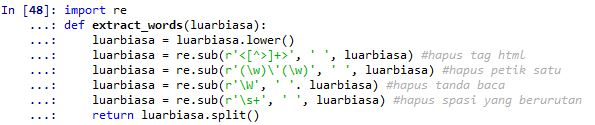
\includegraphics[width=1\textwidth]{figures/huda/chapter5/20.JPG}}
	\caption{Extract\_Words}
	\label{c5_20}
\end{figure}
\subitem PermuteSentences berfungsi untuk melakukan pengacakan data supaya memperoleh data yang teratur. Ini merupakan class yang digunakan untuk melakukan pengocokan secara acak pada data yang ada. Digunakan cara ini agar tidak terjadi kelebihan memori pada saat dijalankan. Hasilnya dapat dilihat pada gambar \ref{c5_21}.
\begin{figure}[!htbp]
	\centerline{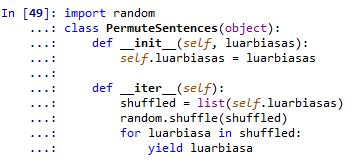
\includegraphics[width=1\textwidth]{figures/huda/chapter5/21.JPG}}
	\caption{Permute Sentences}
	\label{c5_21}
\end{figure}
\item Jelaskan fungsi dari librari gensim TaggedDocument dan Doc2Vec disertai praktek pemakaiannya.
\subitem Fungsi dari library gensim yaitu sebagai pemodelan topik tanpa pengawasan dan pemrosesan bahasa alami, atau bisa kita sebut dengan unsupervised.  tagged document itu sendiri untuk memasukan kata-kata pada setiap dokumennya yang akan di vektorisasi. Fungsi dari doc2vec itu sendiri ialah untuk membandingkan bobot data yang terdapat pada dokumen lainnya, apakah kata-kata didalamnya ada yang sama atau tidak. Ketika di running maka tidak terjadi apa-apa, seperti pada gambar \ref{c5_22}
\begin{figure}[!htbp]
	\centerline{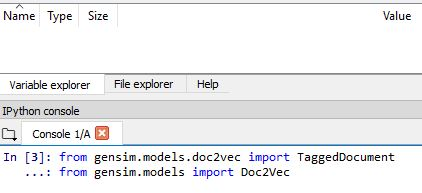
\includegraphics[width=1\textwidth]{figures/huda/chapter5/22.JPG}}
	\caption{Gensim TaggedDocument dan Doc2vec}
	\label{c5_22}
\end{figure}
\item Jelaskan dengan kata dan praktek cara menambahkan data training dari file yang dimasukkan kepada variabel dalam rangka melatih model doc2vec.
\subitem Untuk menambahkan data training yaitu melakukan import library os, library os berfungsi untuk melakukan interaksi antara python dengan os laptop kita masing-masing, setelah itu kita buat variabel unsup sentences. Kemudian pilih direktori tempat data kita disimpan. Lalu menyortir data yang terdapat pada folder aclImdb dan membaca file tersebut dengan ektensi .txt.
\begin{verbatim}
import os
unsup_sentences = []
for dirname in ["train/pos","train/neg","train/unsup","test/pos","test/neg"]:
for fname in sorted(os.listdir("aclImdb/"+dirname)):
if fname[-4:] == '.txt':
with open("aclImdb/"+dirname+"/"+fname,encoding='UTF-8') as f:
sent = f.read()
words = extract_words(sent)
unsup_sentences.append(TaggedDocument(words,[dirname+"/"+fname]))
\end{verbatim}
\subitem Hasil dari code yang diatas ialah terdapatnya data training dengan jumlah 10000 data dari variabel unsup\_sentences hasil running dari folder aclImdb dapat dilihat pada gambar \ref{c5_23}
\begin{figure}[!htbp]
	\centerline{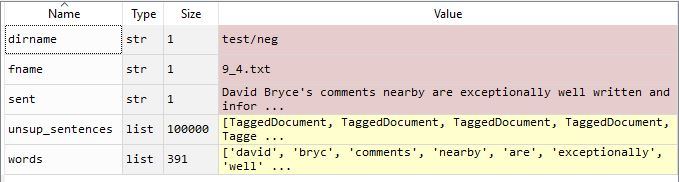
\includegraphics[width=1\textwidth]{figures/huda/chapter5/23.JPG}}
	\caption{Aclimbdb}
	\label{c5_23}
\end{figure}
\begin{verbatim}
for dirname in ["review_polarity/txt_sentoken/pos","review_polarity/txt_sentoken/neg"]:
for fname in sorted(os.listdir(dirname)):
if fname[-4:] == '.txt':
with open(dirname+"/"+fname,encoding='UTF-8') as f:
for i, sent in enumerate(f):
words = extract_words(sent)
unsup_sentences.append(TaggedDocument(words,["%s/%s-%d" % (dirname,fname,i)]))
\end{verbatim}
\subitem Untuk code berikutnya akan menambahkan data training pada variabel unsup\_sentences sekitar 64.720 data, seperti pada gambar \ref{c5_24}
\begin{figure}[!htbp]
	\centerline{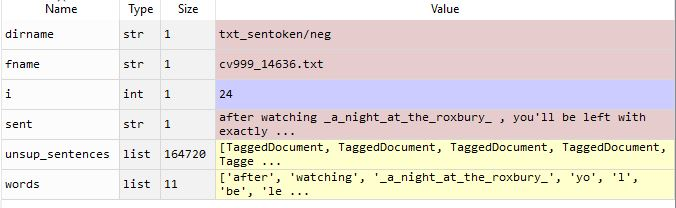
\includegraphics[width=1\textwidth]{figures/huda/chapter5/24.JPG}}
	\caption{Aclimbdb}
	\label{c5_24}
\end{figure}
\begin{verbatim}
with open("stanfordSentimentTreebank/original_rt_snippets.txt",encoding='UTF-8') as f:
for i, sent in enumerate(f):
words = extract_words(sent)
unsup_sentences.append(TaggedDocument(words,["rt-%d" % i]))
\end{verbatim}
\subitem Untuk code berikutnya akan menambahkan data training pada variabel unsup\_sentences sekitar 10.605 data, seperti pada gambar \ref{c5_25}
\begin{figure}[!htbp]
	\centerline{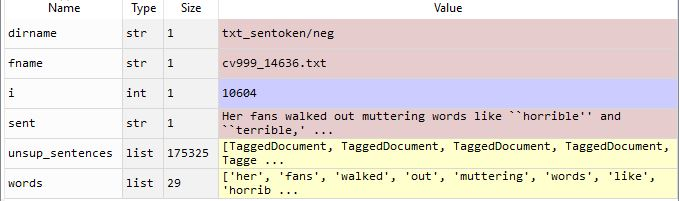
\includegraphics[width=1\textwidth]{figures/huda/chapter5/25.JPG}}
	\caption{Aclimbdb}
	\label{c5_25}
\end{figure}
\item Jelaskan dengan kata dan praktek kenapa harus dilakukan pengocokan dan pembersihan data.
\subitem Pengocokan data itu berguna untuk mengacak data supaya pada saat data di running bisa berjalan lebih baik dan hasil presentase akhirnya bisa lebih bagus. Sedangkan pembersihan data untuk memberikan ruang bagi ram komputer kita setelah melakukan running data sebanyak 3 juta lebih, agar lebih ringan saat proses selanjutnya. Hasil dari pengacakan data tidak ditampilkan pada spyder. Dan sebelumnya memori yang terpakai itu sekitar 87\% , setelah dikosongkan jadi 71\%. Untuk source codenya dapat dilihat sebagai berikut:
\begin{verbatim}
# Pengocokan data
mute = PermuteSentences(unsup_sentences)
# Pembersihan data
model.delete_temporary_training_data(keep_inference=True)
\end{verbatim}
\item Jelaskan dengan kata dan praktek kenapa model harus di save dan kenapa temporari training harus dihapus.
\subitem Save data untuk menyimpan file hasil dari proses training data sebelumnya, model tersebut dilakukan penyimpanan untuk memberikan keringanan pada ram agar saat kita akan melakukan training lagi, model tersebut tinggal di muat saja tanpa harus melakukan traning dari awal dan bisa menghemat waktu. Sedangkan untuk delete temporary training data untuk menghapus data training yang sebelumnya sudah dilakukan dan disimpan, tujuannya memberikan keringanan pada ram. Karena setelah melakukan proses training, ram biasanya jadi berat untuk membaca sampai komputer kita jadi lemot. Untuk source codenya dapat dilihat sebagai berikut:
\begin{verbatim}
# Save data
model.save('ocean.d2v')
# Delete temporary data
model.delete_temporary_training_data(keep_inference=True)
\end{verbatim}
\item Jalankan dengan kata dan praktek maksud dari infer code.
\subitem Infer vector yaitu membandingkan kata yang tercantum dengan vektor pada dokumen yang sudah di muat sebelumnya. Selain itu infer\_vector juga menghitung vektor dari kata yang dicantumkan pada model yang telah kita buat. Seharusnya kata yang dicantumkan itu lebih panjang lagi agar hasilnya bisa lebih baik lagi.
\begin{verbatim}
model.infer_vector(extract_words("I will go home"))
\end{verbatim}
\subitem Pada source code tersebut menghasilkan keluaran seperti pada gambar \ref{c5_26}.
\begin{figure}[!htbp]
	\centerline{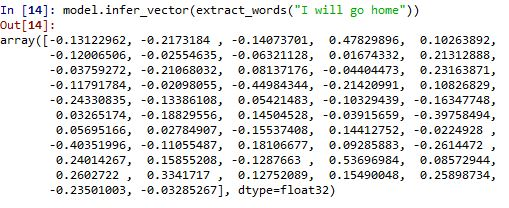
\includegraphics[width=1\textwidth]{figures/huda/chapter5/26.JPG}}
	\caption{Infer Code}
	\label{c5_26}
\end{figure}
\item Jelaskan dengan praktek dan kata maksud dari cosine similarity.
\subitem Cosine similarity yaitu membandingkan vektorisasi data diantara kedua kata yang di masukkan, Jika hasil presentase dari kedua kata tersebut lebih dari 50 persen kemungkinan kata tersebut terdapat dalam 1 file. Tapi jika kurang dari 50 persen kata tersebut tidak terdapat dalam 1 file. Hasil yang didapatkan pada code tersebut hanya 0.4 persen itu dikarenakan kata pertama dan kedua tidak memiliki kesamaan vektorisasi dan tidak terdapat pada salah satu dokumen.
\begin{verbatim}
from sklearn.metrics.pairwise import cosine_similarity
cosine_similarity(
[model.infer_vector(extract_words("she going to school, after wash hand"))],
[model.infer_vector(extract_words("Services sucks."))])
\end{verbatim}
\subitem Pada source code tersebut menghasilkan keluaran seperti pada gambar \ref{c5_27}.
\begin{figure}[!htbp]
	\centerline{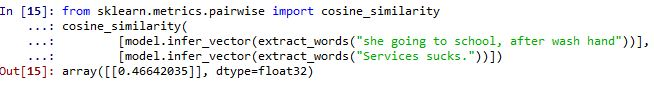
\includegraphics[width=1\textwidth]{figures/huda/chapter5/27.JPG}}
	\caption{Cosine Similarity}
	\label{c5_27}
\end{figure}
\item Jelaskan dengan praktek score dari cross validation masing-masing metode.
\subitem score dari cross validation yang mana mengecek data score KNN untuk menghasilkan typedata float64 dimana terdapat 5 data dari score yang typedatanya float64 tersebut. Dan disini menggunakan metode clf
\begin{verbatim}
scores = cross_val_score(clf, sentvecs, sentiments, cv=5)
np.mean(scores), np.std(scores)
\end{verbatim}
\subitem Pada source code tersebut menghasilkan keluaran seperti pada gambar \ref{c5_28}.
\begin{figure}[!htbp]
	\centerline{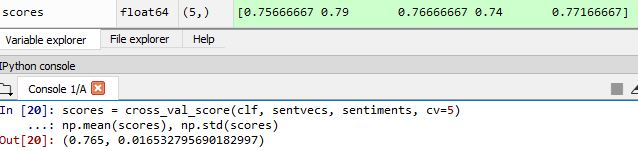
\includegraphics[width=1\textwidth]{figures/huda/chapter5/28.JPG}}
	\caption{Cross Validation Metode 1}
	\label{c5_28}
\end{figure}
\begin{verbatim}
scores = cross_val_score(clfrf, sentvecs, sentiments, cv=5)
np.mean(scores), np.std(scores)
\end{verbatim}
\subitem Pada source code tersebut mengecek data score RF dengan menggunakan metode clfrf yang menghasilkan keluaran seperti pada gambar \ref{c5_29}.
\begin{figure}[!htbp]
	\centerline{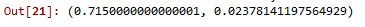
\includegraphics[width=1\textwidth]{figures/huda/chapter5/29.JPG}}
	\caption{Cross Validation Metode 2}
	\label{c5_29}
\end{figure}
\begin{verbatim}
from sklearn.pipeline import make_pipeline
from sklearn.feature_extraction.text import CountVectorizer, TfidfTransformer
pipeline = make_pipeline(CountVectorizer(), TfidfTransformer(), RandomForestClassifier())
scores = cross_val_score(pipeline,sentences,sentiments, cv=5)
np.mean(scores), np.std(scores)
\end{verbatim}
\subitem Pada source code tersebutcmelakukan skoring dari vektorisasi, tfidf, dan rf lalu dibuat perbandingan yang menghasilkan keluaran seperti pada gambar \ref{c5_30}.
\begin{figure}[!htbp]
	\centerline{
\includegraphics[width=1\textwidth]{figures/huda/chapter5/30.JPG}}
	\caption{Cross Validation Metode 3}
	\label{c5_30}
\end{figure}
\end{enumerate}